%
%	Theorieteil
%

\pagebreak
\section{Management of Container Platforms in the Enterprise}

\onehalfspacing

\subsection{Key requirements in Enterprise IT}

A crucial component of security when running container in production, according to NIST, is separation\footnote{Vgl. \textit{Souppaya, M. (2017)}: Application Container Security Guide \cite{sp800-190}}.

Many enterprises will end up with more than one Kubernetes cluster, sometimes with many more.

\begin{figure}[h]
\centering
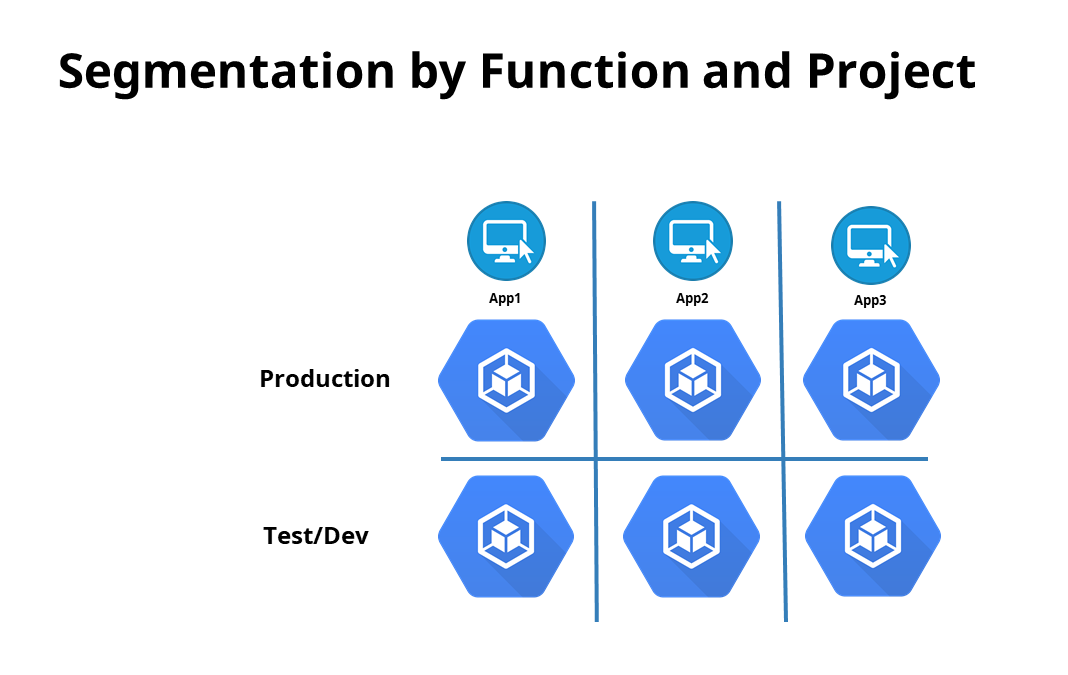
\includegraphics[width=\linewidth]{images/separation}
\caption {Cluster Separation}
\label{fig:clusterSeparation}
\end{figure}

\subsection{Issues when running multiple Kubernetes clusters}

If you run more than one cluster, you'll need to synchronise a lot of tasks across all these clusters

\begin{itemize}
\item User Authentication
\item Roles and Responsibilities
\item Security Policies
    \begin{itemize}
    \item Pod Security Policies
    \item Network Security Policies
    \end{itemize}
\item Applications
\item Versions
    \begin{itemize}
    \item Cluster 
    \item Applications
    \end{itemize}
\end{itemize}

to name a few

Also, you might want to connect your software development pipeline to the various Kubernetes clusters or install a service mesh

\subsection{Possible solutions}

Kubernetes provides a multi-cluster controller, but it's still in its infancy.

Google have Anthos\footnote{Vgl. \textit{Google (2019)}: Anthos - Bringing the cloud to you \cite{googleAnthos}} to address this issue, Microsoft have Azure Arc\footnote{Vgl. \textit{Microsoft (2019)}: Bring Azure services and management to any infrastructure \cite{azureArc}} in Preview

An Open-Source solution for this problem is Rancher\footnote{Vgl. \textit{Rancher Labs (2019)}: Run Kubernetes Everywhere \cite{rancher}}, by Rancher Labs.
